\documentclass[12pt]{article}
\usepackage[utf8]{inputenc}
\usepackage[letterpaper, portrait, margin=1in]{geometry}
\usepackage{amssymb}
\usepackage{amsmath}
\usepackage{graphicx}
\usepackage{tcolorbox}

\newcommand{\example}[1]{\noindent\textbf{Example #1\quad}}
\newcommand{\exercise}[1]{\noindent\textbf{Exercise #1\quad}}
\newcommand{\problem}[1]{\noindent\textbf{Problem #1\quad}}

\pagenumbering{arabic} % arabic, roman, Roman, alph, Alph, gobble
%\setcounter{page}{0} % sets the initial page

\setlength{\parindent}{0pt}
\setlength{\parskip}{10pt}
\setlength{\baselineskip}{15pt}
\linespread{1.2}

\font\sf = cmss10

\usepackage{fancyhdr}
\pagestyle{fancy}
\fancyhf{}
\lhead{MATH 180 Notes}
\rhead{Section 5.1: Areas and Distances}
\rfoot{Page \thepage}
%\thispagestyle{empty}


\begin{document}

Q: How do we find the area of irregular shape?

\begin{tabular}{ll}
\begin{tabular}{l}
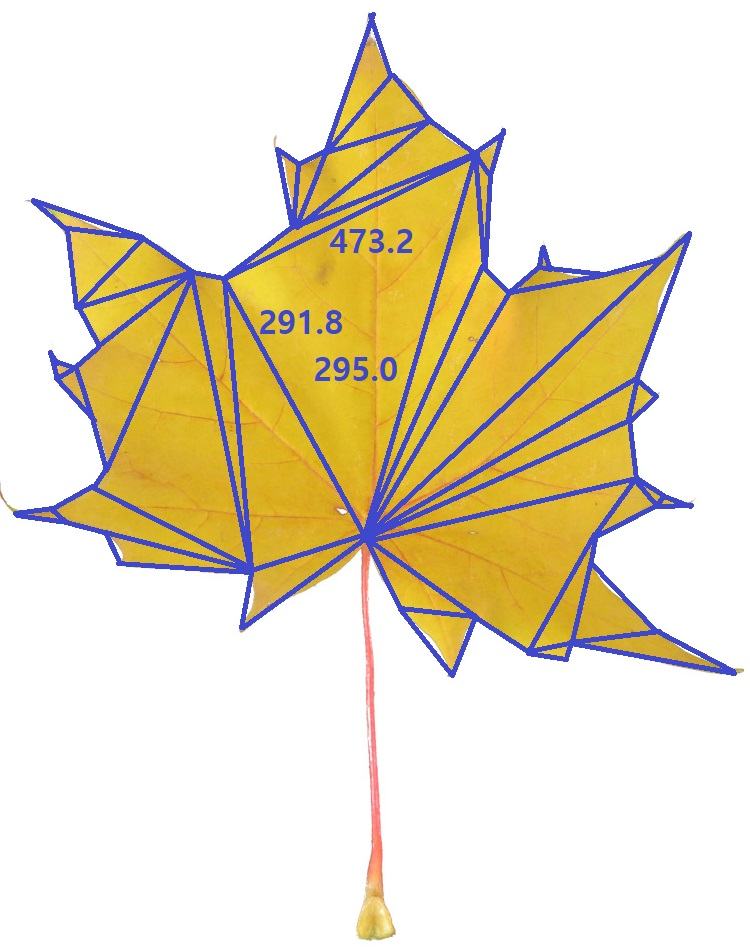
\includegraphics[scale=0.5]{mapleleaf.png}
\end{tabular} & \begin{tabular}{l}
A: Triangularization! The area of the\\
leaf can be found by adding the areas of\\
smaller triangles. For a smaller triangle,\\
we can find the area if we can measure\\
three sides.\\
\\
One of the triangles is measured to have \\
$291.8$, $295.0$, and $473.2$. Using Heron's \\
formula, we can find the area.\\
\\
\textbf{Heron's Formula} for a 
triangle $\triangle ABC$ \\
with the sides lengths $a$, $b$, and $c$: \\
\\
Semi-perimeter: $s = (a+b+c)/2$ \\
Area: $A = \sqrt{s(s-a)(s-b)(s-c)}$ \\
\\
$s = (291.8 + 295.0 + 473.2)/2 = 530$ 
\end{tabular}
\end{tabular}

$$ A = \sqrt{530(530-291.8)(530-295.0)(530-473.2)} = \sqrt{1685131608} = 41050.4 $$

\textbf{Goal}: We want to estimate the area between a curve of a function and $x$-axis.

For instance, what is the area underneath the portion of the sine graph from $x = 0$ to $x = \pi$.

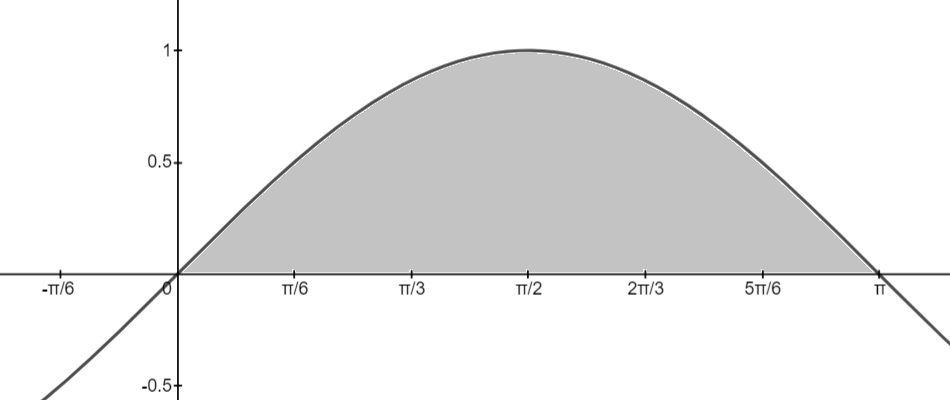
\includegraphics[scale=0.7]{math180_sec5_1_img1.png}

We can get the estimate of the area by using one really large triangle connecting $(0,0)$, $(\frac{\pi}{2},1)$, and $(\pi,0)$, which yields 
the area $\approx \frac{1}{2}(\pi)(1) = 1.5708$. This estimate is clearly underestimation as there are some leftover area not covered by the triangle.
We can make a better esti-\\
\begin{tabular}{ll}
\begin{tabular}{l}
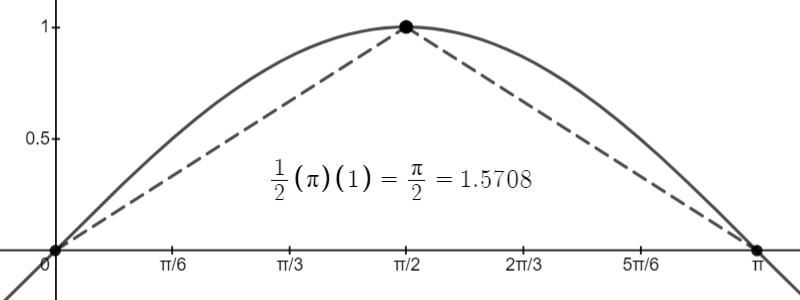
\includegraphics[scale=0.7]{math180_sec5_1_img2.png}
\end{tabular} & \begin{tabular}{l}
mate if we can fur-\\
ther triangularize \\
the leftover areas. \\
More triangles are\\
used, better the esti-\\
mate will be.\\
\\
\end{tabular}
\end{tabular}

Although there are many algorithms for triangularizing a shape out there, it is still far from being simple enough to be formulated as a formula. The next shape we can consider to estimate the area is a quadrilateral (four-sided shape). Especially a rectangle. Its area is simple. \\
\begin{tabular}{ll}
\begin{tabular}{l}
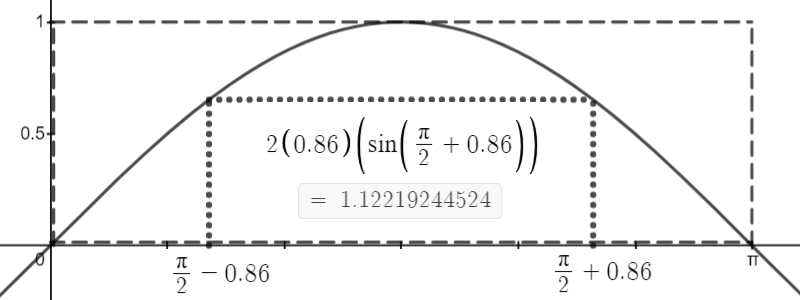
\includegraphics[scale=0.7]{math180_sec5_1_img3.png}
\end{tabular} & \begin{tabular}{l}
We can consider two\\
rectangles. The most\\
obvious rectangle is\\
the one that has the\\
region inscribed, and\\
its area is $(\pi)(1) = \pi$.\\
The other one is the
\end{tabular}
\end{tabular} \\
rectangle with the maximum area that is inscribed in the region, and its area is $2(0.86)(\sin(\frac{\pi}{2} + 0.86)) = 1.1222$. One is an overestimate, and the other is a underestimate.

\textbf{Last Suggestion}: How about using more than one rectangle? We start with four rectangles.

\hspace{50pt}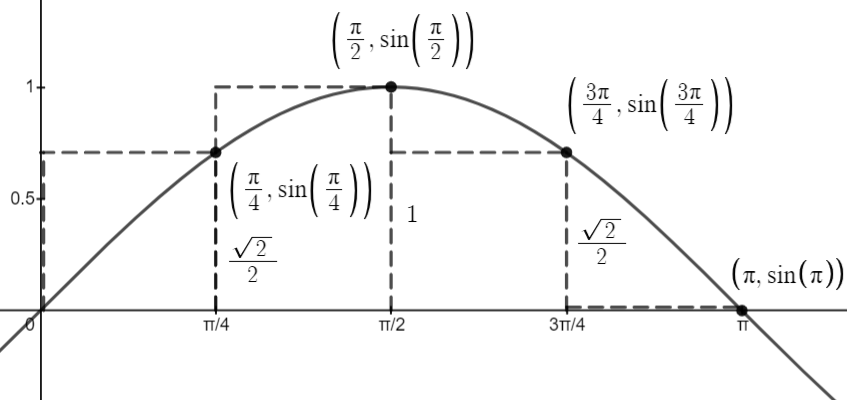
\includegraphics[scale=0.7]{math180_sec5_1_img4.png}

We first partition the real number line from $x = 0$ to $x = \pi$ into
four equal lengths, so the markers of the partition are
$x = 0$, $x = \frac{\pi}{4}$, $x = 2 \cdot \frac{\pi}{4} = \frac{\pi}{2}$,
$x = 3 \cdot \frac{\pi}{4} = \frac{3\pi}{4}$, and $x = 4\cdot \frac{\pi}{4} = \pi$. Above the closed intervals $[0, \frac{\pi}{4}]$, $[\frac{\pi}{4}, \frac{\pi}{2}]$, $[\frac{\pi}{2}, \frac{3\pi}{4}]$, and $[\frac{3\pi}{4}, \pi]$, imagine four rectangles drawn so that the portion underneath the curve of $\sin(x)$ over the closed interval $[0, \pi]$ can be estimated.

Q: How do we determine the height of a rectangle?

There could be infinitely many ways to determine the height of each rectangle, but for the sake of ``consistency,'' we use the right-end number of each closed interval to determine the height of the rectangle. For instance, for the closed interval $[0, \frac{\pi}{4}]$, the right-end number is $\frac{\pi}{4}$. Then we draw a rectangle whose top is drawn passing through the point $(\frac{\pi}{4}, \sin(\frac{\pi}{4}))$ over the closed interval $[0, \frac{\pi}{4}]$. The area of such a rectangle is $(\frac{\pi}{4} - 0)\sin(\frac{\pi}{4}) = \frac{\pi}{4} \cdot \frac{\sqrt{2}}{2} = \frac{\sqrt{2}\pi}{8}$. For the rest of the intervals, if we use the right-end number to determine the height, then 
$$ \text{Area} \approx \left(\frac{\pi}{4} - 0\right)\sin\left(\frac{\pi}{4}\right)
+ \left(\frac{\pi}{2} - \frac{\pi}{4}\right)\sin\left(\frac{\pi}{2}\right)
+ \left(\frac{3\pi}{4} - \frac{\pi}{2}\right)\sin\left(\frac{3\pi}{4}\right)
+ \left(\pi - \frac{3\pi}{4}\right)\sin\left(\pi\right) $$
Since we divide the closed interval $[0,\pi]$ into four equal lengths, the
base of the rectangle should be all $\frac{\pi}{4}$. Then
\begin{eqnarray*}
\text{Area} &\approx & \frac{\pi}{4} \cdot \sin\left(\frac{\pi}{4}\right)
+ \frac{\pi}{4} \cdot \sin\left(\frac{\pi}{2}\right)
+ \frac{\pi}{4} \cdot \sin\left(\frac{3\pi}{4}\right)
+ \frac{\pi}{4} \cdot \sin\left(\pi\right)  \\
&=& \frac{\pi}{4}\left(\sin\left(\frac{\pi}{4}\right) + \sin\left(\frac{\pi}{2}\right) + \sin\left(\frac{3\pi}{4}\right) + \sin\left(\pi\right)\right)  \\
&=& \frac{\pi}{4}\left(\frac{\sqrt{2}}{2} + 1 + \frac{\sqrt{2}}{2} + 0 \right)  \\ &=& \frac{\pi(1 + \sqrt{2})}{4} \quad (\approx 1.8961)
\end{eqnarray*}
The first two rectangles overestimated the region, but last two rectangles underestimated. Just from an inspection of the graph, it seems that we underestimated the region overall. 

Q: How can we improve the estimate?

One can imagine that the portion being overestimated and underestimated can be reduced if we use more rectangles. So let us use $n$ rectangles.

\textbf{Markers}: First, we need to partition the closed interval $[0, \pi]$ into $n$ equal closed intervals. The first marker will be $0$, and let us use the notation $x_0 = 0$ (initial number). Then the second marker will be $x_1 = \frac{\pi}{n}$. The next one is $x_2 = \frac{\pi}{n} + \frac{\pi}{n} = 2 \cdot \frac{\pi}{n}$. The next one is $x_3 = \frac{2\pi}{n} + \frac{\pi}{n} = 3 \cdot \frac{\pi}{n}$. In this way, the very last one would be $x_n = n \cdot \frac{\pi}{n} = \pi$. For instance, if we use $n = 16$ rectangles, the markers are $x_0 = 0$, $x_1 = \frac{\pi}{16}$, $x_2 = \frac{2\pi}{16}$, $x_3 = \frac{3\pi}{16}$, $\ldots$, and $x_{16} = \frac{16\pi}{16} = \pi$.

\textbf{Intervals}: There are $n$ closed intervals starting from $[x_0,x_1]$, $[x_1, x_2]$, $[x_2,x_3]$, $\ldots$, $[x_{n-1}, x_n]$ or
$[0, \frac{\pi}{n}]$, $[\frac{\pi}{n}, \frac{2\pi}{n}]$, $[\frac{2\pi}{n}, \frac{3\pi}{n}]$, $\ldots$, $[\frac{(n-1)\pi}{n}, \frac{n\pi}{n}]$.

\textbf{Base}: The base of the rectangle should be all equal to $\frac{\pi}{n}$.

\textbf{Heights}: If we use the right-end number from each closed interval, the heights are given by $\sin(x_1)$, $\sin(x_2)$, $\sin(x_3)$, $\ldots$, $\sin(x_n) $ or
$$ \sin\left(\frac{\pi}{n}\right), \sin\left(\frac{2\pi}{n}\right), \sin\left(\frac{3\pi}{n}\right), \ldots, \sin\left(\frac{n\pi}{n}\right) $$

\textbf{Area}: Finally the area would be
$$ R_n = \frac{\pi}{n}\left(\sin\left(\frac{\pi}{n}\right) + \sin\left(\frac{2\pi}{n}\right) + \sin\left(\frac{3\pi}{n}\right) + \cdots + \sin\left(\frac{n\pi}{n}\right)\right) $$
The letter $R$ stands for the ``right-end,'' and $n$ represents the number of the rectangles. Before, we found out that
$$ R_4 = \frac{\pi(1 + \sqrt{2})}{4} \approx 1.8961 \quad \text{and} \quad R_6 = \frac{\pi(2 + \sqrt{3})}{6} \approx 1.9541 $$
Here are some more of estimates for different $n$ values with a help from WolframAlpha:

\begin{tabular}{|c|c|l|l|}
\hline
$n$ & $R_n$ & WolframAlpha command & Symbol from WolframAlpha \\
\hline
10 & 1.98352 & (Pi/10)*Sum[Sin[k*(Pi/10)],{k,1,10}] & $\frac{\pi}{10}\sum_{k=1}^{10} \sin(k \cdot \frac{\pi}{10})$ \\
100 & 1.99984 & (Pi/100)*Sum[Sin[k*(Pi/100)],{k,1,100}] & $\frac{\pi}{100}\sum_{k=1}^{100} \sin(k \cdot \frac{\pi}{100})$ \\
500 & 1.99999 & (Pi/500)*Sum[Sin[k*(Pi/500)],{k,1,500}] & $\frac{\pi}{500}\sum_{k=1}^{500} \sin(k \cdot \frac{\pi}{500})$ \\
\hline
\end{tabular}

Q: Any guess on what this estimate will be close to as $n \to \infty$?

\subsubsection*{Sigma Notation}

Instead of writing
$$ R_{10} = \frac{\pi}{10}\left(\sin\left(\frac{\pi}{10}\right) 
+ \sin\left(2 \cdot \frac{\pi}{10}\right) 
+ \sin\left(3 \cdot \frac{\pi}{10}\right) 
+ \cdots 
+ \sin\left(10 \cdot \frac{\pi}{10}\right)\right) $$
we can write using $\Sigma$ (capital letter `sigma' in Greek alphabet) notation.
$$ R_{10} = \frac{\pi}{10}\boxed{\sum_{k = 1}^{10} \sin\left(k \cdot \frac{\pi}{10}\right)} $$
It is a succinct way of writing a sum of many expressions that has some patterns that can be described in a nice expression. The sigma notation is written as
$$ \sum_{\text{running index } = \text{ beginning index value}}^{\text{ending index value}} \text{expression usually involving the running index} $$ 
Then the notation represents the sum of the expression by evaluating the expression with the running index starting from the beginning index value to the ending index value ``incrementing by 1.'' For instance,
$$ \sum_{k = 1}^{10} k = 1 + 2 + 3 + 4 + 5 + 6 + 7 + 8 + 9 + 10 $$
$$ \sum_{k = 1}^{10} (2k + 1) = (2\cdot 1 + 1) + (2 \cdot 2 + 1) + (2 \cdot 3 + 1) + \cdots + (2\cdot 10 + 1) $$
$$ \sum_{k = 6}^{10} \pi = \pi + \pi + \pi + \pi + \pi $$
Then
$$ R_n = \frac{\pi}{n}\sum_{k = 1}^n \sin\left(k \cdot \frac{\pi}{n}\right) $$ 
The area under the curve of $y = \sin(x)$ over the closed interval $[0, \pi]$ is best estimated by
$$ \lim_{n \to \infty} R_n = \lim_{n \to \infty} \frac{\pi}{n}\sum_{k = 1}^n \sin\left(k \cdot \frac{\pi}{n}\right) \text{ which we suspected to be } 2 $$ 


\example{1} Find the area under the curve of $y = \sin(x)$ over the closed interval $[\frac{\pi}{3}, \frac{5\pi}{6}]$.

\hspace{50pt}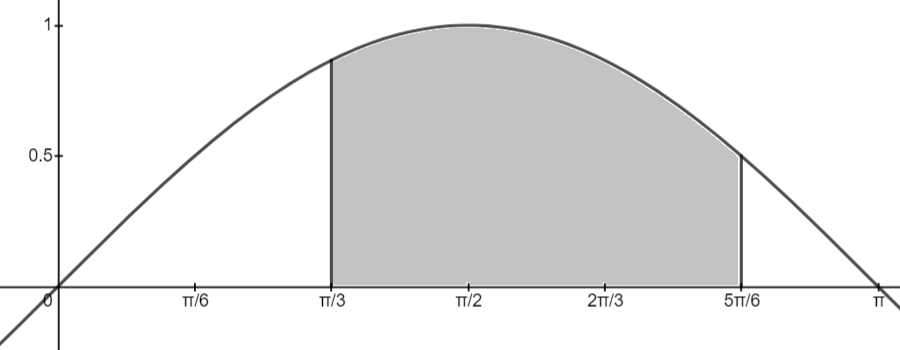
\includegraphics[scale=0.7]{math180_sec5_1_img5.png}

Let us try $n = 10$ rectangles. The equal width of the interval is obtained by
$$ \Delta x = \frac{\text{length of the closed interval}}{n} = \frac{\frac{5\pi}{6} - \frac{\pi}{3}}{10} = \frac{\pi}{20} $$
\textbf{Markers}: The first marker is $x_0 = \frac{\pi}{3}$ (not zero any longer). The second marker is $x_1 = \frac{\pi}{3} + \frac{\pi}{20}$. The next marker is $x_2 = \frac{\pi}{3} + 2 \cdot \frac{\pi}{20}$. The rest are
$$ x_3 = \frac{\pi}{3} + 3 \cdot \frac{\pi}{20}, \quad x_4 = \frac{\pi}{3} + 4 \cdot \frac{\pi}{20}, \quad  \ldots,  \quad x_9 = \frac{\pi}{3} + 9 \cdot \frac{\pi}{20},  \quad x_{10} = \frac{\pi}{3} + 10 \cdot \frac{\pi}{20} $$
\textbf{Intervals}: The closed intervals are $[x_{k-1}, x_k]$ where $k = 1, 2, \ldots, 10$ or\\
$[\frac{\pi}{3} + (k-1) \cdot \frac{\pi}{20}, \frac{\pi}{3} + k \cdot \frac{\pi}{20}]$ where $k = 1, 2, \dots, 10$.

\textbf{Base}: $\Delta x = \frac{\pi}{20}$.

\textbf{Heights}: Using the right-end number, the height is $\sin(\frac{\pi}{3} + k \cdot \frac{\pi}{20})$ where $k = 1, 2, \ldots, 10$. 

\textbf{Area}: The area is estimated using
$$ R_{10} = \frac{\pi}{20} \sum_{k = 1}^{10} \sin\left(\frac{\pi}{3} + k \cdot \frac{\pi}{20}\right) \approx 1.33447 $$

\subsubsection*{Right-End Rectangle (RER)}

There is nothing special about $\frac{\pi}{3}$, $\frac{5\pi}{6}$, $\sin(x)$, or $n = 10$.
Suppose that we want to estimate the area under the curve of $y = f(x)$ over the closed interval $[a, b]$ using $n$ rectangles.

\textbf{Base}: The equal length of the closed intervals is 
$$ \boxed{\quad \Delta x = \frac{b-a}{n}\quad} $$
\textbf{Markers}: $x_0 = a$, $x_1 = a + \Delta x$, $x_2 = a + 2\cdot \Delta x$, $\ldots$, $x_n = a + n \cdot \Delta x = b$. Or
$$ \boxed{\quad x_k = a + k \cdot \Delta x, \text{ where } k = 1, 2, \ldots, n \quad} $$
\textbf{Heights}: $f(x_1)$, $f(x_2)$, $f(x_3)$, $\ldots$, $f(x_n)$. Or
$$ \boxed{\quad f(x_k) = f(a + k \cdot \Delta x) \quad} $$
\textbf{Area}: The area is estimated using
$$ \boxed{\quad R_n = \Delta x \sum_{k = 1}^n f(x_k) = \Delta x \sum_{k=1}^n f(a + k \cdot \Delta x)\quad} $$
This is called the \textbf{right-end rectangle} estimate $R_n$.

\example{2} Find the area under the curve $f(x) = x^2$ over the closed interval $[2, 5]$.
Use $n = 6$ rectangles.

\textbf{Base}: The equal length of the closed intervals is $\Delta x = \frac{5-2}{6} = \frac{1}{2}$

\textbf{Markers}: $x_0 = 2$, $x_1 = 2 + \frac{1}{2}$, $\ldots$, $x_6 = 2 + 6 \cdot \frac{1}{2} = 5$.\\
Or $x_k = 2 + k \cdot \frac{1}{2} = 2 + \frac{k}{2}$ where $k = 1, 2, 3, 4, 5, 6$.

\textbf{Heights}: $f(x_k) = (x_k)^2 = (2 + \frac{k}{2})^2$

\textbf{Area}: The area is estimated using the right-end rectangle estimate
\begin{eqnarray*}
R_6 &=& \frac{1}{2} \sum_{k=1}^6 \left(2 + \frac{k}{2}\right)^2 \\
&=& \frac{1}{2}\left(\left(2 + \frac{1}{2}\right)^2
+\left(2 + \frac{2}{2}\right)^2
+\left(2 + \frac{3}{2}\right)^2
+\left(2 + \frac{4}{2}\right)^2
+\left(2 + \frac{5}{2}\right)^2
+\left(2 + \frac{6}{2}\right)^2\right) \\
&=& \frac{355}{8} \quad = \quad 44.375
\end{eqnarray*}








\vfill


Assigned Exercises: 


\end{document}